	La GDT (\textit{Global Descriptor Table}) es una estructura de datos
que la arquitectura Intel x86 utiliza para almacenar distintos descriptores
de sistema, como descriptores de segmento ordinarios o descriptores de Task State 
Segment (TSS). Estos permiten asignar características o propiedades a distintas secciones de la memoria, 
o permiten identificar la ubicación y atributos de diferentes estructuras necesarias para el funcionamiento 
del sistema.
	En la primer entrada de la tabla siempre se asigna un descriptor nulo, por requerimiento del 
sistema de protección. El procesador produce una excepción automáticamente cuando se intenta acceder a la posición cero de la GDT.

\subsection{Descriptores de segmento y Segmentación flat}

	Los descriptores de segmento delimentan el tamaño y la ubicación de los segmentos de memoria, así como 
sus propiedades: quién los puede acceder, que clase información alojan (datos o código), entre otras. De esta forma, permiten particionar el espacio de memoria para ser utilizado por diferentes actores y con diferentes utilidades, garantizando que no se viole la integridad del esquema mediante el sistema de protección.

	El mecanismo de segmentación optado en este trabajo consiste en una segmentación tipo flat.
Este mecanismo consiste en anular virtualmente la protección por segmentación que provee la arquitectura, armando segmentos superpuestos entre sí, ocupando la totalidad de la memoria. Se configuraron cuatro segmentos: dos con nivel de privilegio 0 (máximo nivel de provilegios), y dos con nivel de privilegio
3 (mínimo nivel de privilegios). Para cada nivel se utilizó un segmento de código y uno
de datos.

\begin{figure}[h]
\begin{center}
  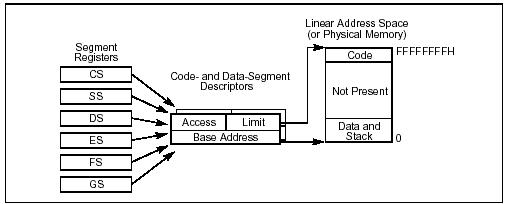
\includegraphics[scale=3.0]{secciones/dibujitos/modelo_flat.jpg}
\end{center}
\caption{Segmentación flat}
\end{figure}

	La decisión de dejar de lado la protección por hardware brindada a través de la segmentación se basa 
en la posibilidad de lograr resultados similares, pero de forma más sencilla y flexible, mediante el mecanismo de paginación, descripto en la próxima sección.

	Otra consecuencia de la segmentación flat es que los descriptores de segmento con sus parámetros 
adecuados se conocen de antemano y se configuran en tiempo de compilación. Una vez que el sistema 
entra en ejecución, estos descriptores de segmento no se vuelven a modificar.

	Adicionalmente, se creó un segmento conteniendo la memoria de video, principalmente con 
fines didácticos ya que el manejo de la pantalla se realizó en su totalidad mediante el segmento de datos de nivel 0.

\subsubsection{Atributos descriptores de segmento}


\begin{figure}[h]
\begin{center}
  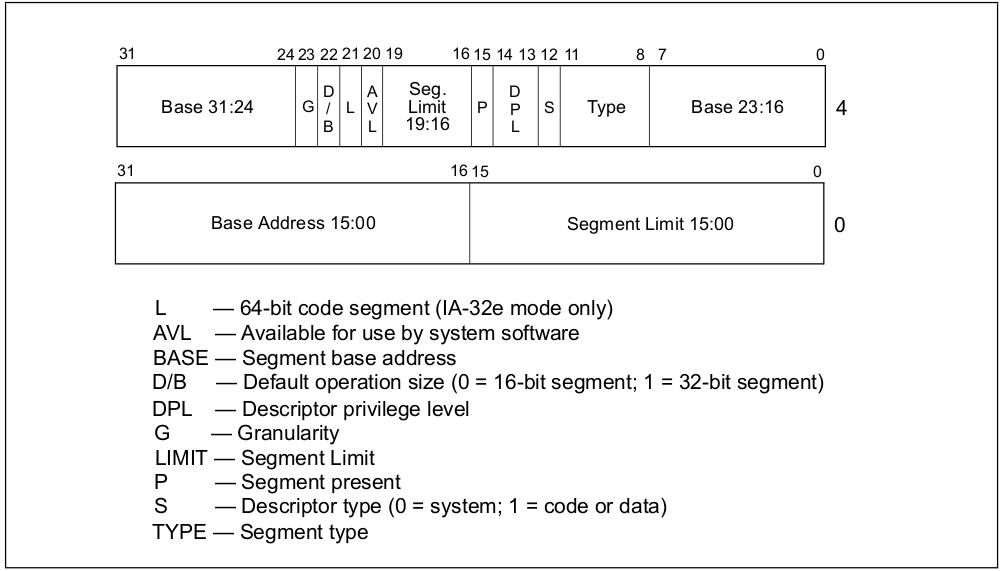
\includegraphics[scale=0.3]{secciones/dibujitos/descriptorDeSegmento.png}
\end{center}
\caption{Descriptor de segmento}
\label{fig:descriptorDeSegmento}
\end{figure}

	
	Al usar sementación flat, la configuración correcta para los atributos para cada segmento es la 
siguiente: la base del segmento debe estar en la posición 0, el límite debe ser el tamaño máximo 
de cada segmento (1,75gb en este caso) menos 1, la granularidad (G) tiene que estar en 1, pues los sectores serán de 4kb, y el bit Present (P) tiene que estar en 1, habilitando el uso del segmento.

	El resto de los parámetros varían en cada segmento; los dos segmentos que serán utilizados por el 
kernel requieren Descriptor Privilege Level (DPL) igual a 0, y los otros dos serán de acceso a nivel usuario con DPL igual a 3. Por último, es necesario especificar el tipo del segmento, ya sea datos o código (uno de cada tipo por cada nivel, como se dijo previamente).

\subsection{Descriptores de TSS}

	Los descriptores de TSS son necesarios para utilizar el cambio automático entre tareas 
que provee la arquitectura. Describen la posición y el tamaño de las estructuras donde se almacena 
el estado de cada tarea del sistema; es decir, el valor de sus registros, la tarea predecesora, y más información.

	El almacenamiento de las TSS se realizó de forma dinámica, sin predeterminar su posición en 
tiempo de compilación. Por eso sus respectivos descriptores deben ser definidos en tiempo de 
ejecución, lo cual se realizó mediante las siguientes funciones en C:

\begin{minted}{c}
	void tss_inicializar_entrada_gdt_tarea_inicial();
	void tss_inicializar_entrada_gdt_idle();
	void tss_inicializar_entrada_gdt_navio(unsigned int nro_tarea);
	void tss_inicializar_entrada_gdt_bandera(unsigned int nro_tarea);
\end{minted}

	Si bien estas funciones tienen mucho en común se las creo por separado
por una cuestión pragmática que sirvió para encontrar errores y \textit{bugs} mas
fácilmente.

	Estas funciones a su vez se engloban todas en otra función escrita en C que
inicializa todas las TSS y se llama desde \textbf{kernel.asm}

\begin{minted}{c}
	void tss_inicializar();
\end{minted}

\begin{comment}
	
	En la GDT hay que poner los descriptores de segmento
y los descriptores de TSS para cada cada tarea y para cada bandera.

	La misma está representada como un arreglo ``$gdt\_entry$'' declarado
de manera global en C. Las $gdt\_entry$ son structs de 4 bytes que poseen un campo
cara cada atributo de una entrada de gdt.

	Los descriptores de segmento fueron cargados de manera estática
en tiempo de compilación. Lo mismo con el descriptor de la IDT. Esto
fue posible porque se conocen de antemano todos los valores
necesarios para completar los descriptores.

	A la hora de cargar los descriptores de TSS nos encontramos con la
siguiente dificultad: Los descriptores de TSS fueron declarados como una
variable global en código C. Por lo tanto en tiempo de compilación
no se sabe en que dirección van a ser cargados. Por este motivo se cargan
de manera dinámica mediante una función que se llama desde kernel.asm. La
función sencillamente crea una entrada más en el arreglo que representa 
de $gdt\_entry$ con los atributos adecuados.
\end{comment}
